\chapter{Design of Experiments}
\chaptermark{DOE}

This chapter is devoted to the matter of designing experiments, and follows the lines of \cite{cox_theory_2000}.
A control chart may be seen as an on-line experiment alerting us when the milk goes sour, but it will not tell us why. 
When designing a product (remember DFSS \ref{sec:dfss}), or once a control chart has signalled an alert, we will want to know what \emph{controllable inputs} influence our process, and how to reduce its variability.
In our SPC terminology, we will want to know what are the \emph{causal} \emph{effects} of our controllable inputs (\emph{factors}), on our \emph{CTQ} (\emph{response}). 
The theory of discovering these effects is the theory of \emph{design of experiments} (DOE).
Its goal is to \emph{screen} factors with no effect, 
to estimate effect sizes, 
find optimal factor-level combinations, 
and remove assignable variability; 
all these as efficiently as possibly.


Several matters should be emphasized:
\begin{description}
\item [Randomization] is the random assignment of units to treatments. 
It is fundamental to our purpose because the idea of an \emph{effect} implies \emph{causality}. 
Since we seek to intervene in the production to reduce variability, we only care about causal effects. 
It is the mechanism of \emph{randomization}, that allows us to conclude that the correlations we find are indeed causal, and not merely statistical.
For a treatment of causal inference in \emph{observational data}, i.e., without randomization, see \cite{rosenbaum_observational_2002}.

\item [Pre-experiment] In this text we take it for granted that the purpose of the experiment is well known, and the candidate factors defined. 
We are fully aware, as should be the reader, that in application this is a non-trivial luxury. 
Indeed, a lot of meetings, planning, and expertise go into the selection of factors, their candidate levels, etc.

\item [Power Analysis] Part of the pre-experiment may include a power analysis. 
The pre-experiment power analysis will typically be very approximate, and rely on many assumptions. 
It is still important, as it gives an idea of the feasibility of an experiment, and avoids wasting resources.

\item [No Textbook Solution] We will present many design ideas and principles, yet in real life problems rarely obey text-books.
You should thus feel free, and even obliged, to think about your particular problem and adapt the experiment as you best see fit. 

\item[Data Analysis]
In this text, we only discuss the \textbf{design} of the experiment, and not the \textbf{analysis} of the data.
This is a non-standard choice as DOE is typically presented alongside the \emph{analysis of variance} (ANOVA) framework.\marginnote{ANOVA}
We decouple the two for several reasons. 
First, because \cite{cox_theory_2000} do so. 
Second, because these are two different thing.
The ANOVA framework may be replaced by the framework of \emph{linear models}, \emph{mixed models}, \emph{variance components}, and possibly others analysis frameworks. 
There is a vast literature focusing on the analysis.
If asked, this author may recommend \cite{hocking_analysis_1985}, which presents both the ANOVA terminology, and the linear models terminology.
That book, however, may be hard to come by, so feel free to ask me for other references if required.

\end{description}




Roughly speaking, the challenges in designing good experiment are:
\begin{enumerate}
\item Efficiency: extract the most information per sampled unit.
\item Signal to noise: reduce variability to reveal factor effects.
\item Bias: correctly identify the (causal) effect of each factor, without ``absorbing'' other effects.
\end{enumerate}
After establishing the required terminology, we will discuss design methods that deal with reduction of the noise, so that factor effects can be better detected and estimated (Section~\ref{sec:variance_components}).
We will then discuss the efficiency of designs. 
In particular, how to represent different treatments in a way that allows a single experimental condition, to be informative not only on itself, but also on other experimental conditions (Section~\ref{sec:factorial_design}).





\section{Terminology}
Many, if not most of the following terms, originate in R.A. Fisher's seminal book ``The Design of Experiments'' \citep{fisher_design_1960}. 
As such, the DOE literature is rich in agricultural terms, due to its historical origins.
When old ideas get new names, we try to emphasize this in the text.


\begin{tcolorbox}[breakable]
\begin{description}

\item [Design]  Complete specification of experimental test runs, including blocking, randomization, repeat tests, replication, and the assignment of factor–level combinations to experimental units.

\item [Experimental Unit]  Entity on which a measurement or an observation is made.

\item [Homogenous Experimental Unit] Units that are as uniform as possible on all characteristics that could affect the response.

\item [Factors]  A controllable experimental variable that is thought to influence the response. 
In the language of SPC: \emph{a controllable input}.

\item [Level] Specific value of a factor.

\item[Treatment] The particular factor-level combination applied to an experimental unit. 
\Aka \emph{manipulation}, or \emph{cell}.

\item [Factor Encodings] 
The numerical encoding of factor levels.
Of minor importance for designing. 
Of major importance for analysis.
Two level factor encodings include:
	\begin{enumerate}
	\item Effect coding: where levels are encoded with $\set{-1,1}$.
	\item Dummy coding: where levels are encoded with $\set{0,1}$.
	\end{enumerate}

\item [Design Matrix] A matrix description of an experiment that is useful for constructing and analyzing experiments.

\item [Response] 
The CTQ in the SPC literature. 
The $y$ variable in the regression literature. 
The \emph{response} in the DOE literature. 

\item [Main Effect] Change in the expected response between two factor–levels.  
We emphasize that effects, unlike simple population parameters, imply a causal relationship.
Akin to the \emph{assignable causes} in the SPC literature, and $\beta$'s in the regression literature. 

\item [Interaction] Existence of joint factor effects in which the effect of each factor depends on the levels of the other factors.
Part of the \emph{assignable causes} in the SPC literature.

\item [Noise] \Aka \emph{error}. 
The variability in the response that cannot be attributed to any factor.
This is the \emph{common} variability in the SPC literature, and the $\varepsilon$ in the regression literature. 

\item [Replication] A single repetition of an entire experiment, i.e., a single measurement of the response in all experimental conditions.

\item [Repeats] Repeated measurements on the response under the same conditions, i.e., under the same treatment. \Aka \emph{repeat tests}.

\item [Covariate]  An variable that influences the response but is unaffected by any other experimental factors.
We cannot change at will, but we can \emph{control/account for them}. 

\item [Non Specific Factor] A variable that we suspect to affect the response, but we can only vaguely define, thus impossible to measure. 
As a consequence, we will not care to study its effect, but rather just remove it (e.g. by blocking). 
Think of ``life style'' as an example of a non-specific factor.

\item [Blocking]  Blocking, or \emph{grouping}, is an experimental design technique that removes excess variation by grouping experimental units or test runs so that those units or test runs within a block are more homogeneous than those in different blocks. Blocking attributes are also known as \emph{non specific factors}.
The blocking in the design needs to be accounted at the time of the data analysis.

\item [Confounding] When the design is such that several effects cannot be told apart. \Aka \emph{aliasing}.

\item [Balance] A vaguely defined concept, capturing symmetry in the combinatorial design of the experiment. 
In its simplest interpretation, a design where an equal number of units is assigned to each treatment.

\end{description}

\end{tcolorbox}







\section{Dealing with Variability}
\label{sec:variance_components}

The idea that random samples come with (common causes of) variability, i.e. noise, should not be new to the reader.
In this section, we will try to decompose variability into it sources, and learn several techniques to reduce them. 
Starting with a motivating example, which you should use to fix ideas as you progress along this chapter. 



\begin{example}[Web Design]
\label{eg:variance_components}
Consider the problem of optimizing a web site, where individuals performance is measured by conversion rate (the probability of a new user to signup, purchase, etc).
In the DOE language, the conversion is the \emph{response}.
A user (or ip address) is an \emph{experimental unit}.
The site's attributes are the \emph{factors}.
A particular site's design, i.e. a combination of factors, is the \emph{treatment}.
The users' attributes are \emph{covariates}. 
The user's life-style, a \emph{non-specific factor}.
If the site's attributes affect differently users with different attributes, we say there is an \emph{interaction}.
\end{example}




\begin{example}[Two Competing Diets]
\label{eg:twins}
Consider the problem of comparing two nutrition diets. 
Clearly, the effect of a diet on life expectancy strongly interacts with both genetics and life style. 
It would be thus very nice if we could block experimental units, so that each block has a homogenous genetics and life-style. 
That is why twins are so popular when designing experiments!
\end{example}




\subsection{Gage R\&R Studies}
R\&R stands for \emph{repeatability} and \emph{reproducibility}.
In the context of quality control\footnote{Beware that these words are used with different meanings by different communities.} repeatability is the variability under \emph{test repeats}, and reproducibility is the variability when the same experiment is performed elsewhere (different lab, technician, etc.).
Gage R\&R experiments are aimed at measuring the precision of an experiment, i.e. its repeatability and reproducibility, by collecting data from different test repeats performed at different labs. 



\subsection{Completely Randomized Designs}
In the simplest of designs, all experimental units are randomly assigned to treatments. 
This is typically easy to implement.
In Example~\ref{eg:variance_components} this would imply randomly assigning users to interfaces.
If you suspect, as you should, that we may reduce variability by grouping types of users together, keep reading.



\subsection{Randomized Block Designs}
The idea of \emph{blocking} is to replace the complete randomization scheme by a restricted randomization scheme so that variability can be reduced without introducing bias. 
The restricted randomization is created by \emph{grouping}, or \emph{blocking} groups of experimental units, and randomizing allocation within the group. 

In our running example, we could reduce the variability of the web site's attributes by showing various sites to the same person- each person would be his own block. This is an example of \emph{crossover} design, discussed in Section~\ref{sec:crossover}.

Alternatively, we could block individuals along, say, using the age covariate. 
We would then randomly assign users to layouts, only within age groups, so that all layouts are presented to each age-group. 
If each age group has as many users as there are different site designs, this is a \emph{randomized complete block design}.\marginnote{Complete Block Design}
If there are more layouts than users in each age group, we cannot randomize all layouts within all age groups. 
This would require an \emph{incomplete block design}.
There are several approaches to incomplete block designs, but we refer the reader to \cite[Sec.4.2]{cox_theory_2000} for details.

The reader may have noticed by now that blocking is done in order to great homogenous groups, thus reducing the variability in measured response. 
One can block using either factors, covariates, or non-specific factors. 


\begin{think}
With twins, you can have a complete block design comparing only two treatments. 
How would you go about to compare three treatments?
\end{think}



\subsubsection{Latin Square Design}
When homogenous groups are defined by two non-specific factors, we would like to create blocks that are balanced, so that the non-specific factors do not bias effect estiamtes.
In our running example, non-specific factors may be age and gender. 
We could construct all age and gender combinations, and randomly assign users from each age-gender to each site design.
This would is an example of a \emph{split plot} design, discussed in Section~\ref{sec:split_plot}.
If, however, we do not deal with age-gender, but rather with age-country, we may not have enough users in each cell to assign to all site designs. 
Since we do not want to estimate the effect of age, nor country, but merely balance the design so that age and country effects do not alias the site's effect, we do not actually need all age-country combinations. 



If we have $k$ designs, we may group ages and countries into $k$ categories each, and each design is seen only once in each age group and once in each country group. 
This allocation of treatment to blocks is known as a \emph{Latin Square}. 
Table~\ref{tab:latin_square} demonstrates a Latin Square for $7$ web site designs, and compares it to a non-balanced allocation. 
\begin{table}[ht]
    \begin{minipage}{.5\linewidth}
        \centering
		\begin{tabular}{rlllllll}
		  \hline
		 & 1 & 2 & 3 & 4 & 5 & 6 & 7 \\ 
		  \hline
		1 & 1 & 2 & 3 & 4 & 5 & 6 & 7 \\ 
		2 & 1 & 2 & 3 & 4 & 5 & 6 & 7 \\ 
		3 & 1 & 2 & 3 & 4 & 5 & 6 & 7 \\ 
		4 & 1 & 2 & 3 & 4 & 5 & 6 & 7 \\ 
		5 & 1 & 2 & 3 & 4 & 5 & 6 & 7 \\ 
		6 & 1 & 2 & 3 & 4 & 5 & 6 & 7 \\ 
		7 & 1 & 2 & 3 & 4 & 5 & 6 & 7 \\ 
		   \hline
		\end{tabular}
    \end{minipage}%
    \begin{minipage}{.5\linewidth}
      \centering
		\begin{tabular}{rlllllll}
		  \hline
		 & 1 & 2 & 3 & 4 & 5 & 6 & 7 \\ 
		  \hline
		1 & 1 & 2 & 3 & 4 & 5 & 6 & 7 \\ 
		  2 & 2 & 3 & 4 & 5 & 6 & 7 & 1 \\ 
		  3 & 3 & 4 & 5 & 6 & 7 & 1 & 2 \\ 
		  4 & 4 & 5 & 6 & 7 & 1 & 2 & 3 \\ 
		  5 & 5 & 6 & 7 & 1 & 2 & 3 & 4 \\ 
		  6 & 6 & 7 & 1 & 2 & 3 & 4 & 5 \\ 
		  7 & 7 & 1 & 2 & 3 & 4 & 5 & 6 \\ 
		   \hline
		\end{tabular}
		\end{minipage} 
	\caption{A $7$-treatment, two-factor design. 
	Left pane is not balanced.
	Right pane is balanced with a Latin Square, generated with the \rcode{MOLS()} function of the \rcode{crossdes} \R package.}
	\label{tab:latin_square}		
\end{table}


The following example makes the same point, with the original agricultural motivation for this design.
\begin{example}[Agricultural Yield Study]
\label{eg:latin_square}
Consider an farmer growing corn.
He wishes to study the effect of $7$ candidate fertilizers (single factor with $7$ levels).
He is aware that the location of the plot may affect yield, due to slightly different sunlight, irrigation, altitude, etc.
He thus assumes he has to deal with two extra variance sources: row and column of the plot. 
He could treat the row and column as two factors, with $7$ levels each, be he does not care to estimate the row/column effect, but merely to avoid bias.
He will thus try to look for an allocation of fertilizer to rows and columns so that any row/column effect will be averaged out.
The Latin Square design of Table~\ref{tab:latin_square} does just that.
\end{example}


\begin{extra}\noindent
\begin{enumerate}
\item If the Latin Square reminds you of Soduko, it should. Soduko is just that!
\item The Latin Square is a very economical design, and is not used as often as it should be.
\item If we had reason to believe that different age groups in different countries respond differently to each site (an interaction), then the Latin Square may actually introduce aliasing. 
\end{enumerate}
\end{extra}



\subsubsection{Extensions of the Latin Square}
\begin{enumerate}
\item \textbf{Latin Hypercube}: When balancing more than two non-specific factors, we will call upon \emph{latin hypercube designs}, \aka \emph{orthogonal latin squares}. \marginnote{Orthogonal Latin Squares}
\item \textbf{Greco-Latin Square}: A latin-hypercube with three variability sources. 
\end{enumerate}






\subsubsection{Crossover Design}
\label{sec:crossover}
Lets return to the web site layout example (\ref{eg:variance_components}).
Let us also assume that our site has $3$ web pages. A landing page, an information page, and a form to fill. 
It is possible that the response to a particular page is affected by the previous page presented. 
This is known as a \emph{carryover effecf}, or \emph{residual effect}, which may bias the main layout effects of interest. \marginnote{Carryover Effect}

The more general phenomenon is dependence in the noise between trials. 
Consider the same subject undergoing different treatments, or adjacent fields. 
\emph{Crossover} designs are such that all possible treatment adjacencies are considered, so that the carry over effect averages out. 

In a \emph{fully randomized crossover design}, each unit is randomly allocated to a sequence of treatments.
If treatments are combinations of several factors, it is not uncommon to use Latin Squares to generate the sequences. Table~\ref{tab:crossover} demonstrates the $3!=6$ sequences for our $3$ page website problem.
\begin{table}[ht]
\centering
\begin{tabular}{rlll}
  \hline
 & 1 & 2 & 3 \\ 
  \hline
1 & 1 & 2 & 3 \\ 
  2 & 2 & 3 & 1 \\ 
  3 & 3 & 1 & 2 \\ 
  4 & 1 & 3 & 2 \\ 
  5 & 2 & 1 & 3 \\ 
  6 & 3 & 2 & 1 \\ 
   \hline
\end{tabular}
\caption[Crossover Design]{Crossover design: a balanced sequence of administration of $3$ treatments, generated with the \rcode{des.MOLS()} function of the \rcode{crossdes} \R package. }
\label{tab:crossover}
\end{table}






\section{Factorial Designs}
\label{sec:factorial_design}
Until now we discussed some arbitrary set of treatments.
It is quite common, is not certain, that the many treatments are merely combination of a small number of \emph{factors} with a small number of \emph{levels} each.
This means that we may decompose treatment effect into the (partial) sums of the effects of underlying factors, which would make both the design more economical, and the analysis easier to interpret.

We will now present several designs for factorial experiments.
Recall that factors define treatments. The noise reducing and bias avoiding methods of Section~\ref{sec:variance_components} may thus be compounded with the treatment generating methods of this section.

It should be emphasized that a factorial design is better than $k$ experiments with one factor at a time. This is because:
\begin{enumerate}
\item Factorial experiments are make better (statistical) use of each sample unit for estimating main effects.
\item Factorial experiments allow the estimation of interactions between factors. 
\end{enumerate}
A classical illustration of the second point, is given in Figure~\ref{fig:one_factor_at_a_time}.
The figure depicts a one-factor-at-a-time optimization sequence (from A to H). Since the factors are not varied simultaneously, the experiments is unable to identify that the response is not a linear surface. 
Put differently, he is unable to estimate an interaction.

\begin{figure}[ht]
\centering
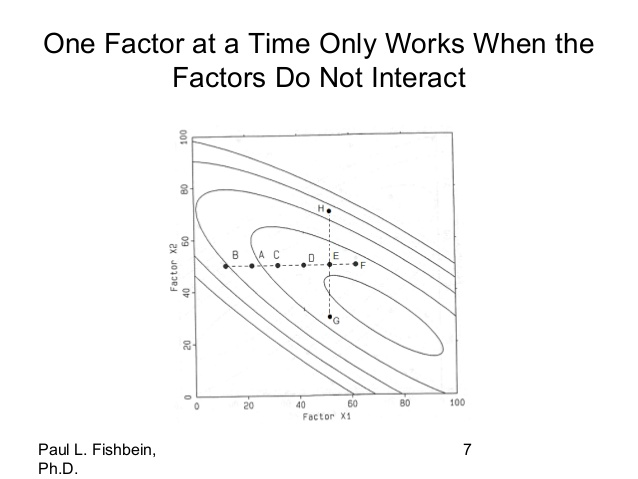
\includegraphics[height=0.3\textheight]{art/optimization-without-statistical-doe-2015-03-23-7-638}
\caption[One-at-a-time optimization]{Optimizing factors, one at a time.\newline \url{http://www.slideshare.net/PaulFishbein/optimization-without-statistical-doe-2015-03-23-46817073}}
\label{fig:one_factor_at_a_time}
\end{figure}




\subsection{Full Factorial Designs}
A \emph{full factorial}, or \emph{complete factorial} design, is one where all factor-level combinations are replicated the same number of times.
The most common of the full-factorial designs is the $2^k$-design where all combinations of $k$ factors with two levels each are tested in each replication.



\subsubsection{$2^k$ design}
Consider two factors denoted $A$ and $B$.
Adopt the effect coding so that we encode their levels by $\set{-1,1}$.
The design matrix of a single run is depicted in Figure~\ref{fig:full_factorial} (top right) along with a visualization of the design (top left).
Allowing $n$ observations per condition, the experiment will include $4n$ observations, which will be randomized between conditions.

\begin{figure}[ht]
\centering
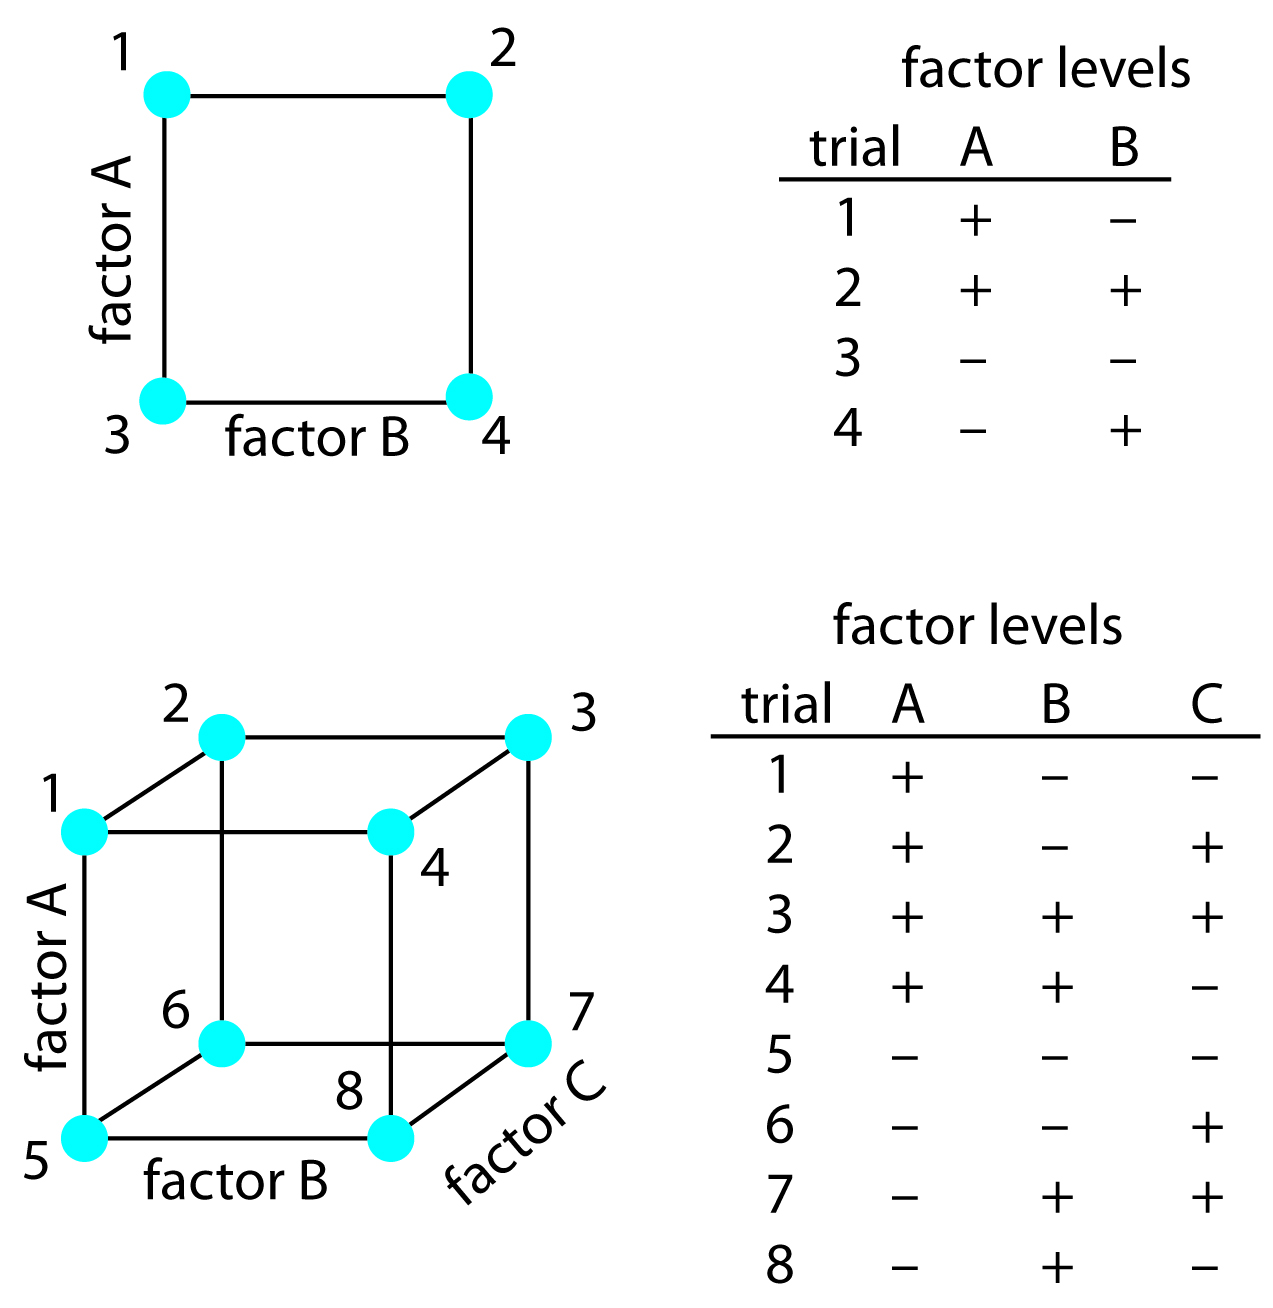
\includegraphics[width=0.7\linewidth, height=0.3\textheight]{art/full_factorial}
\caption[Full Factorial Design]{Full factorial designs: $2^2$ and $2^3$. \newline \url{http://chemwiki.ucdavis.edu/Analytical_Chemistry/Analytical_Chemistry_2.0/14_Developing_a_Standard_Method}}
\label{fig:full_factorial}
\end{figure}
With this $2^2$ design, we may recover several effects:
\begin{description}
\item [Main effect of A] The effect of varying $A$ from $(-)$ to $(+)$.
\item [Main effect of B] The effect of varying $B$ from $(-)$ to $(+)$.
\item [Main effects and interaction] The effect of varying both $A$ and $B$ from $AB=(--)$ to $AB=(++)$.
\end{description}

We typically denote the (mean) response for each treatment by the $\mu_{\smiley}$ notation, where $\smiley$ encodes the applied treatment by stating the conditions that were at their $+$ state:
\begin{table}[H]
\centering
\begin{tabular}{|c|c|c|c|}
\hline Treatment & A & B & Mean \\ 
\hline 1 & + & - & $\mu_a$ \\ 
\hline 2 & + & + & $\mu_{ab}$ \\ 
\hline 3 & - & - & $\mu_{(1)}$ \\ 
\hline 4 & - & + & $\mu_b$ \\ 
\hline 
\end{tabular} 
\end{table}

\marginnote{Interaction}

Slightly intruding into the realm of data analysis, a visualization of interactions is known as the \emph{interaction plot}, depicted in Figure~\ref{fig:interaction_plot}. 
The upper left panel demonstrates a lack of interaction (think why), while the upper right panel depicts an interaction.
\begin{figure}[ht]
\centering
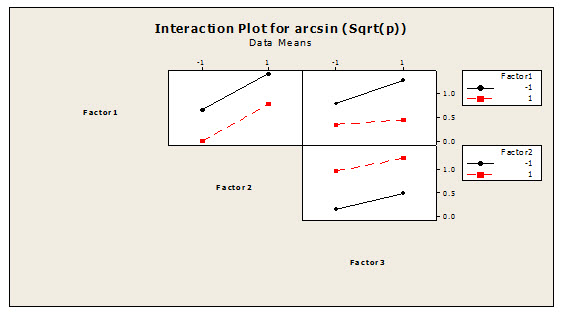
\includegraphics[width=0.3\textheight]{art/attribute_doe_interaction_plot}
\caption[Interactions plot]{Interactions plot. \newline \url{http://blog.minitab.com/blog/statistics-in-the-field/optimizing-attribute-responses-using-design-of-experiments-doe-part-2}}
\label{fig:interaction_plot}
\end{figure}


\begin{remark}[Screening Experiments]
The $2^k$ designs are probably the most popular full factorial designs. 
This may be attributed to the fact that many factors studied really have two levels, but more plausibly, since these are merely \emph{screening} experiments. 
Once non related factors have been screened, the experimenter may proceed from the $2^k$ design to more elaborate ones. 
\end{remark}



\begin{remark}[Intermediate Factor Levels]
In a $2^k$ design, a factor may actually be a continuous controllable input which was restricted to two values for convenience. 
After estimating the effect of the factor, we may want to know what the effect would have been, had we set it on some intermediate level.
It is customary to assume that a main effect acts linearly in-between experimental conditions, yet you should remember that there is nothing in the data to support this.
For a more rigorous approach, see the Response Surface Methodology Section (\ref{sec:response_surface}).
\end{remark}


\begin{remark}[Crossed Treatments]
Both crossover designs and full factorial designs are \emph{crossed} in that all factor combinations are sampled. 
The difference is that in a full-factorial, a factor combination is applied simultaneously to an experiment unit, and in a crossover design, the application is sequential \citep{everitt_cambridge_2010}.
\end{remark}



\subsubsection{$3^k$ Designs}
I think that the name $3^k$ design is rather self explanatory.
Then again, more than $2$ levels are rarely treated as factorial experiments. 
This is because $3$ level factors typically appear when aiming at optimizing the factor combination, for which the \emph{response surface} methodology of Section~\ref{sec:response_surface} is more economical.




\subsection{Fractional Factorial}
Full factorial designs are the simplest designs to setup and interpret. 
A major drawback, are the resources required when $k$ is large. 
This is where the \emph{fractional factorial}, or \emph{partial factorial} designs kick in.
The fundamental idea is to design a full factorial, but skip a couple experimental conditions. If conditions to skip are wisely selected, only information on higher order interactions will be compromised.


\begin{example}[From $2^2$ to $2^{2-1}$]
\label{eg:fractional_factorial}
As a first toy example, we will try to save some time and money by eliminating particular conditions of the $2^2$ design in Figure~\ref{fig:full_factorial}.
As the name may suggest, a $2^{2-1}$ design, has $2$ experimental conditions in each run. 
There are thus $\binom{4}{2}=6$ possible eliminations, which are enumerated in Table~\ref{tab:partial_factorial} along with the extractable information in each elimination.
\begin{table}[ht]
\begin{tabular}{|p{2.5cm}|p{10cm}|}
\hline Elimination &  Problem \\ 
\hline
\hline 1,2 &  No information on $a$. \\ 
\hline 1,3 &  No information on $b$.\\ 
\hline 1,4 &  $a$ aliased with $b$ aliased with $ab$. \\ 
\hline 2,3 &  $a$ aliased with $b$ aliased with $ab$. \\ 
\hline 2,4 &  No information on $b$. \\ 
\hline 3,4 &  No information on $a$.\\ 
\hline 
\end{tabular} 
\caption[Aliasing]{Aliasing in a $2^{2-1}$ design: All possible eliminations from the $2^2$ design that lead to a $2^{2-1}$ design.}
\label{tab:partial_factorial}
\end{table}
\end{example}

The lesson from Example~\ref{eg:fractional_factorial} is that in a fractional factorial our savings in time and money, come at the cost of the information that can be drawn from the experiment.
The idea behind partial factorial experiments, is that by an informed choice of the conditions skipped, we can choose what information to give up. The information lost, is known as the \emph{alias structure}.\marginnote{Alias Structure}

In practice, we will rarely go over all the $\binom{2^k}{2^k-2^{k-p}}$ possible eliminations of conditions, but rather revert to pre-selected designs. 
Table~\ref{tab:partial_factorial_ii}, generated with the \rcode{FrF2()} in the \rcode{FrF2} \R package, is an optimal $2^{5-2}$ design.
Using the \rcode{design.info()} function of that same package, we know that the aliasing structure of this design is
$a=bd=ce, b=ad, c=ae, d=ab, e=ac$.
We will not go into the details of how the aliasing structure is computed, but rather refer the reader to \cite{cox_theory_2000}.
\begin{table}[ht]
\centering
\begin{tabular}{rrrrrr}
  \hline
 & A & B & C & D & E \\ 
  \hline
1 & -1 & 1 & -1 & -1 & 1 \\ 
  2 & 1 & -1 & 1 & -1 & 1 \\ 
  3 & -1 & -1 & -1 & 1 & 1 \\ 
  4 & -1 & 1 & 1 & -1 & -1 \\ 
  5 & -1 & -1 & 1 & 1 & -1 \\ 
  6 & 1 & 1 & 1 & 1 & 1 \\ 
  7 & 1 & -1 & -1 & -1 & -1 \\ 
  8 & 1 & 1 & -1 & 1 & -1 \\ 
   \hline
\end{tabular}
\caption[Fractional Factorial Design]{$2^{5-2}$ design.}
\label{tab:partial_factorial_ii}
\end{table}




\begin{definition}[Resolution of a Design]
In previous versions of this text I defined the \emph{resolution} of a design. 
Since my definition was wrong, you are kindly asked to ignore it.
\end{definition}

\begin{tcolorbox}
\paragraph{My mistake!}
The previous definition is plain wrong. 
It is thus removed from the course's syllabus until I update it.
\end{tcolorbox}



\begin{extra}[Coding Theory]
There is a close relationship between design of experiments and coding theory in computer science. 
A possible reference on the matter is \cite{hill_first_1986}, or \cite{hedayat_orthogonal_1999}.
\end{extra}



\subsection{Split Plot Design}
\label{sec:split_plot}
Revisiting our web site layout problem:
We want to block along age and country. 
For each age and country combination (full factorial blocking) we can randomly assign users to site layouts. 
This combination of a factorial design for blocking, is known as a \emph{split plot}, or \emph{split unit} design.
For more on split plots see \cite[Sec.6.4]{cox_theory_2000}.

\subsection{Summary of Discrete Factors}
In this section we dealt with discrete factors, typically taking two possible values.
These appeared for several purposes. 
The most obvious way, was to define treatments: in full factorial, and fractional factorial designs, the treatments are decomposed into their defining factors. 
Decomposing treatments to their factors allowed us to be more economical in our designs (think why?).
Factors were, however, also encountered when reducing variability. 
When used for defining blocks, or groups, we called these non-specific factors simply because all we required for grouping was some vague notion of homogeneity within a block, and not an explicit definition of the factor that defines the blocks. 

In the next section, we extend from discrete factors to continuous factors.

\section{Continuous Factors}
When dealing with \emph{continuous factors}, or \emph{quantitative factors}, we have many more analysis strategies than when dealing with qualitative factors.
No matter the analysis strategy, it is still important of choosing the right factor level combinations to study.

Clearly, we cannot identify nonlinearities when sampling a factor only a two levels.
We may thus opt for a full $3^k$ factorial design to fit a non-linear surface to the data.
The factor encoding would typically be $\{-1,0,1\}$,
A full $3^k$ factorial design may however be needlessly expensive. 
A more common approach in industrial application is the \emph{central composite design}, where a $2^k$ design is augmented with well chosen sampling points. \marginnote{Central Composite Design}
For more details see \cite[Sec.6.6]{cox_theory_2000}


\subsection{Response Surface Methdology}
\label{sec:response_surface}
As the name suggests, \emph{response surface methdology} deals with the estimation of the response surface to the levels of continuous factors.
Response surfaces are typically assume to be (approximately) quadratic, and experimentation typically conducted in stages. First screening factors, then fitting a surface, and finding optimal factor levels.



\subsection{Taguchi Methods}
\emph{Taguchi methods} is a collective name for the philosophy, design, and analysis methods in industrial applications promoted by Genichi Taguchi in 1970's Japan.
Focusing on the design principles, we may note the following particularities of Taguchi's method:
\begin{enumerate}
\item Achieving low variability is more challenging then achieving a target value. 
\item Factors which can be controlled in a lab, but not in production, are deliberately varied. Typically with split plot  designs (\ref{sec:split_plot}).
\item Systematic use of latin hypercubes to study main effects and two-way interactions. Particularly \emph{Plackett–Burman designs}.\marginnote{Plackett Burman Design}
\item Log variability ($\log s$) is often used as the response.
\end{enumerate}





\section{Optimal Designs}
% 1D least squares example
% pD least squares example
% logistic regression example


Our discussion until now has been informal with respect to the desirable qualities of a design. 
We used the idea of ``balance'' and ``orthogonality'' to avoid bias and unwelcome variability.
In this section, we try to formalize the notion of a ``good design''.
We start with some motivating examples.

\begin{example}[Design for linear regression]
\label{eg:design_linear}
Figure~\ref{fig:design_linear} demonstrates the effect of the different location of the sampling points ($x$) on the quality of the estimated regression line, in a \textbf{linear} model.
As the figure depicts, and intuition suggests, it is preferable to spread the sampling points as far as possible.
\begin{figure}[ht]
\centering
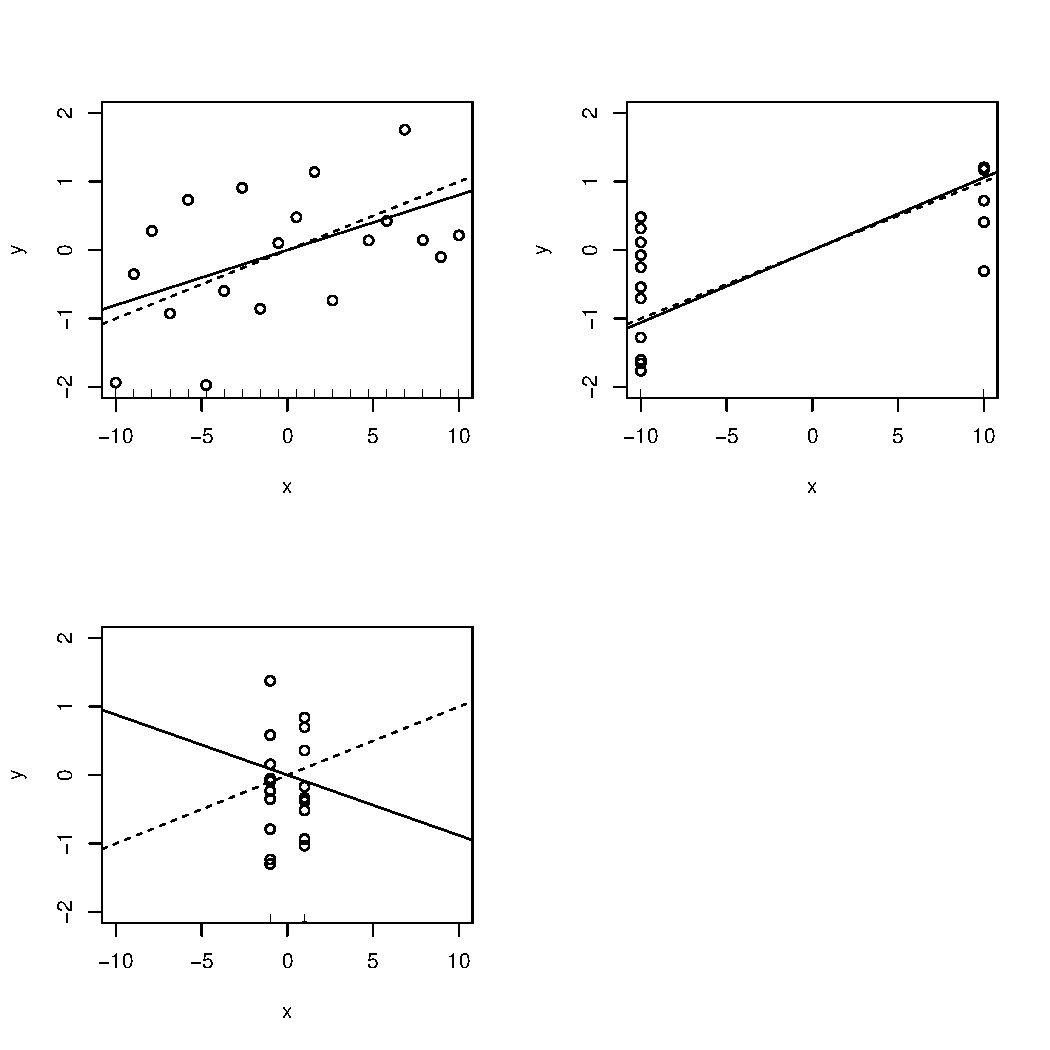
\includegraphics[height=0.3\textheight]{art/linear}
\caption[Design for Linear Models]{Design for linear regression. Different panels show different designs. True function as a dashed line. Estimated function as a full line.}
\label{fig:design_linear}
\end{figure}
\end{example}





\begin{example}[Design for non linear regression]
\label{eg:design_non_linear}
Figure~\ref{fig:design_nonlinear} demonstrates the effect of the different location of the sampling points ($x$) on the quality of the estimated regression line, in a \textbf{nonlinear} model.
It may seems that unlike the linear case (Example~\ref{eg:design_linear}) optimality is achieved in some intermediate spread of the $x$s.
\begin{figure}[ht]
\centering
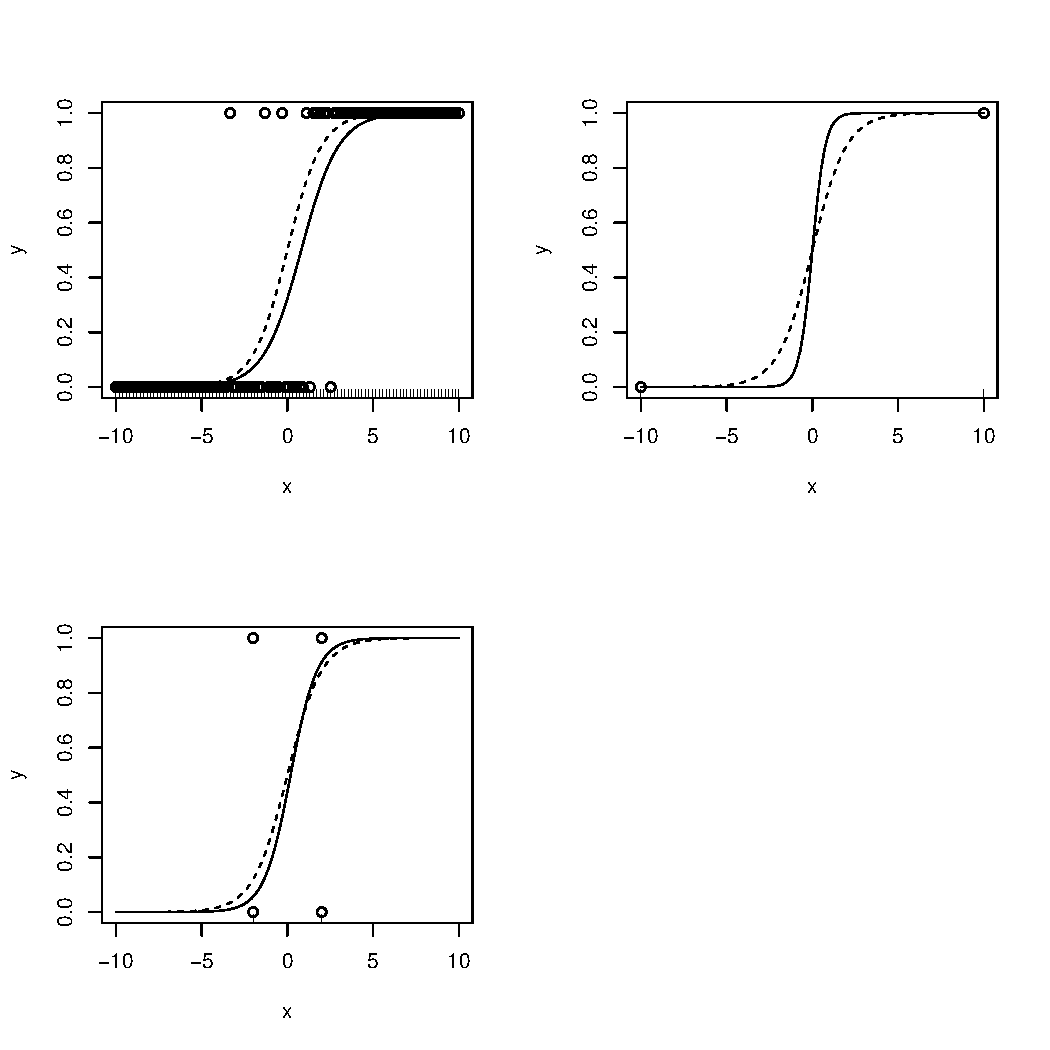
\includegraphics[height=0.3\textheight]{art/nonlinear}
\caption[Design for Non Linear Models]{Design for non linear regression. Different panels show different designs. True function as a dashed line. Estimated function as a full line.}
\label{fig:design_nonlinear}
\end{figure}
\end{example}





Now for some facts, supported by the previous examples:
\begin{enumerate}
\item The idea of ``balancing'' as a design criterion is very useful with discrete factors, but limited with continuous factors. 
\item The optimal design may depend on the unknown generative model. Luckily, for linear models, this is not the case, and an optimal design will be so for all values of the generative parameter.
\end{enumerate}



\subsection{Space Filling Design}
\label{sec:space_filling}
The most natural of designs, which is particularly suitable when we have no a-priori assumption on the functional relation ($f(x)$) between the (continuous) factors and the response, is known as a \emph{space filling design}.
As the name suggests, in a space filling design we aim at filling the factor space. Lacking any a-priori information, the filling will typically be as uniform as possible. 
We note however, that once information on $f(x)$ is made available, then a space filling design is typically sub optimal (see Example~\ref{eg:design_linear}).


\begin{extra}[Space Filling and Hashing]
If you are familiar with the idea of \emph{hashing functions}, then you may see the similarity between space filling and the \emph{uniformity} property of hash functions. 
For a more rigorous discussion, see \cite{hill_first_1986}.
\end{extra}



\subsection{Covariance Optimality}
We have already noted the the optimality of the design depends on the data generating process.
In this section it is made obvious that optimality will also depend on the analysis method we choose.

When estimating the effect of a single continuous factor, we would like a design that gives us the most information per observation on some effect $\beta$. 
This is the same as minimizing the variance of the estimator, $\min \{Var[\hat{\beta}]\}$, with respect to the design.
In the case of linear regression with a single coefficient we know that 
\begin{align}
	Var[\hat{\beta}] &= \frac{\sigma^2_\varepsilon}{\sum_{i=1}^{n}(x_i-\bar{x})^2}.
\end{align}
Minimizing $Var[\hat{\beta}]$ is thus the same as spreading the $x$'s as far as possible, in accordance with the intuition from Example~\ref{eg:design_linear}.
Now recall that in a multivariate linear regression problem with an $n \times p$ design matrix, then 
\begin{align}
	Var[\hat{\beta}] &= \sigma^2_\varepsilon (X'X)^{-1}.
\end{align}
In this multivariate case, there may be several notions of ``maximal spread''. 
Denoting $M:= (X'X)^{-1}$, we can define:
\begin{definition}[A-Optimality]
	A design is said to be \emph{A optimal} if it minimizes the average univariate variance.
	Formally: $\min \set{\Tr(M)}$.
\end{definition}
A-optimality does not account for covariances. 
In an extreme scenario, if we have several copies of the same variable, the more copies we have, the more importance that variable will be given by A-optimality.
The most popular optimality criterion is known as \emph{D-optimality}, and does not suffer from this phenomenon.
\begin{definition}[D-Optimality]
	A design is said to be \emph{D optimal} if it minimizes the volume of the confidence region for $\beta$. 
	Formally: $\min \set{\det(M)}$.
\end{definition}

Both A-optimality and D-optimality implicitly target linear models, such as in Example~\ref{eg:design_linear}, because they aim at spreading the $x$'s. From Example~\ref{eg:design_non_linear} we know this to be sub-optimal doe non-linear designs. 
For non-linear designs, one may opt for space filing designs (\ref{sec:space_filling}), or consult \cite{pukelsheim_optimal_1993}. 



\begin{extra}[Other Optimality Criteria]
There are as many optimality criteria as there are matrix norms. For a more detailed review, see \cite{wikipedia_optimal_2015}.
For a mathematical rigorous, and through treatment, see \cite{pukelsheim_optimal_1993}.
\end{extra}







\section{Sequential Designs}
\label{sec:sequantial}
% Mark Vandelmeulenbruke

Consider a clinical trial with a treatment and control group.
Now assume the medicine being tested is a miracle cure with immediate improvement. 
Do we really need to keep administering placebos to the control group, just because that was the initial experimental design?
This is where sequential designs come in.
Interestingly, the initial application of a sequential design was not in drug testing, but rather in a military context \citep{wald_sequential_1945}.

The problem with sequential testing, is the \emph{type-I error inflation}, which is simply a \emph{multiplicity problem}. \marginnote{Multiplicity}
To see this, think about an endless sequential experiment. Also assume the null hypothesis is true. 
Because of consistency, then a regular (non sequential) experiment will not reject $H_0$?
But if the test is sequential, the type-I error of endlessly many tests at level $\alpha$ each, will certainly be making more than $\alpha$ mistakes (unless dependence is perfect).

In it simplest version, a sequential design allows early stopping for rejection of the null, or for futility (non-rejection). 
In more elaborate schemes then not only is early stopping allowed, but also the redesign of the experiment. 
This is known as \emph{adaptive design}. The crux, as usual, is not inflating the type-I error, or introducing bias, by redesigning.\marginnote{Adaptive Design}

\begin{extra}[Active Learning]
In the machine learning literature, the idea of adaptive design of experiments is known as \emph{active learning}, where the emphasis is less on adaptive-testing, but rather on adaptive-estimation.
\end{extra}




\subsection{Pooled Designs}
\emph{Pooled designs}, \aka as \emph{group testing} appears when it is cheaper to measure the response for a group of experimental units simultaneously, rather then for each single one. 
It originated in the context of identifying soldiers with syphilis in WWII. It was the Harvard Economist Robert Dorfman that suggested \cite{dorfman_detection_1943} that one may mix blood samples from several soldiers and then repeat the same in the subgroups that show the presence of syphilis. 
The method became immensely popular in the DNA analysis age, where technology allows biologists to test for the presence of particular protein in a sample from a group of cells (e.g. a blood sample). 

Pooled designs broadly classify into two classes: 
\begin{description}
\item [Adaptive group testing] Where the groupings, and the groups to be tested depend on the previous results in the same experiment (see also \emph{adaptive designs}).
\item [Non-adaptive group testing] Where the experiment consists of sequential group tests, but the design is fixed independently of the experimental results. 
\end{description}


\begin{extra}[Bloom filters]
If you are familiar with data structures and particularly \emph{Bloom Filters}, then you will probably note that a Bloom filter is a data structure that groups objects in a way that facilitates lookup using group testing. 
\end{extra}



\section{$A\backslash B$ Testing}
Our web-site optimization example is interesting not only because it accommodates so many DOE practices, but it is also a practical problem of great interest.
For historical reasons, the experimentation with several web-site layouts is not called a factorial experiment (which it is), but rather an \emph{$A\backslash B$-test}.

Some particular characteristics of $A\backslash B$ testing include:
\begin{enumerate}
\item Users come by the millions. Sample size is rarely an issue, so that avoiding bias is more important than avoiding variability.
\item Browser cookies, or login details define blocks. Technology permits to optimize the size for each block separately. If blocking is to very specific subgroups (female users, running Linux, that purchased on Amazon, etc.), then sample size, and thus variability, may become an issue again.
\item Sites have many layout parameters (locations, colours, sizes,...). Studying all these combinations may result on a formidable task (full factorial?!?).
\end{enumerate}




\section{Computer Experiments}
% no randomness
% space filling parameter choices for simulation
\begin{example}[Designing Wings]
\label{eg:wings}
Consider the problem of designing an air-craft's wing.
We would like to know how the wing's attributes, i.e., factors, govern its lift.
We could obviously conduct real-life experiments by varying the wing's attributes, building the wing, flying the air-plane, and recording results. 
Needless to say how expensive this process is.
It is much more reasonable to program the differential equations that govern the lift to a computer, fix several factors values, and solve the equations.
This is what \emph{computer experiments} are all about. 
\end{example}


The wind design example (\ref{eg:wings}) demonstrates the following points:
\begin{enumerate}
\item Computer experiments are essentially numerical solutions to complicated systems of equations.
\item Because solutions take a lot of time, only a small finite set of factor levels may be evaluated. 
\item The ``response'' to each treatment, is deterministic. 
\item The problem of interest is in reconstructing the response at non measured factor levels, so that optimal values may be identified. 
\end{enumerate}
It is thus not uncommon to call upon DOE theory for choosing the factor combinations to be experimented with. Space filling designs (Sec.~\ref{sec:space_filling}) being a particularly prevalent choice. 
The analysis of computer experiment is very different than real-life experiment since we have no noise component. 
See \cite{sacks_design_1989} or \cite{santner_design_2013} for further details. 



\section{Bibliographic Notes}
For an overview of DOE see \cite{cox_theory_2000}, \cite{mason_statistical_2003}, \cite{everitt_cambridge_2010}. 
Another nice and freely available resource is a Penn State course on the topic\footnote{\url{https://onlinecourses.science.psu.edu/stat503/node/1}}. 
Some seminal references in the field include \cite{fisher_design_1960} and \cite{box_statistics_1978}.
For causal inference in non-designed experiments see \cite{rosenbaum_observational_2002}. 
For optimal designs see \cite{pukelsheim_optimal_1993}.
For analysis of data: linear models, ANOVA, etc.\ there are endlessly many books. This author's recommendations include \cite{hocking_analysis_1985}, \cite{greene_econometric_2003}. 
For the relation between factorial designs and coding theory in computer science, see \cite{hill_first_1986}. 
For design and analysis of computer experiments, see \cite{sacks_design_1989} or \cite{santner_design_2013}.
